\documentclass[12pt]{exam}		%Doc : https://mirrors.ircam.fr/pub/CTAN/macros/latex/contrib/exam/examdoc.pdf
\printanswers					%Comment this line to hide the answers 
\usepackage[utf8]{inputenc}
\usepackage[T1]{fontenc}
\usepackage[french]{babel}      %Originally for french document, change to english or relevant language

\usepackage{amsmath,amssymb}
\usepackage{multicol}
\usepackage[dvipsnames]{xcolor}
\usepackage[shortlabels]{enumitem}
\usepackage{tikz}
	\usetikzlibrary{fadings}
	\usetikzlibrary{calc}
	
\usepackage{tkz-tab}
\usepackage{pgfplots}

%Format Header and footer
\pagestyle{headandfoot}
\header{\footnotesize Class\\Id number}{\Large\textbf{Name}}
\headrule
\footrule
\setlength{\columnsep}{0.25cm}
%\setlength{\columnseprule}{1pt}
\footer{}{Page \thepage}{}
%\extrafootheight{-2cm}

% Change section command behaviour
\usepackage{titlesec}
\titleformat{\section}[frame]{\Huge\bfseries\filright}{}{2mm}{\centering Chemistry 123 :\ }

% Add a watermark if answers are shown
%\ifprintanswers
%\usepackage{draftwatermark}
%\SetWatermarkColor{red!30}
%\SetWatermarkScale{5}
%\SetWatermarkText{Solution}     %Watermark text
%\fi

%Format the name of each exercise
\qformat{\textbf{Exercice \thequestion~:}\hfill}
\extrawidth{1.5cm}

\begin{document}
\section{Final Exam B}

\noindent The 68 pts exam consists of 7 questions and students have the whole class period to complete the exam.
Answers must be written in the box provided or else no credit is provided. Use the empty
space provided to do your work. A periodic table is provided at the end. Fill in your name along with your
student ID number.
\\

\noindent\textbf{Problem 1: Sulfur Phase Diagram} Answer the following questions for the
phase diagram of sulfur. (4 pts)

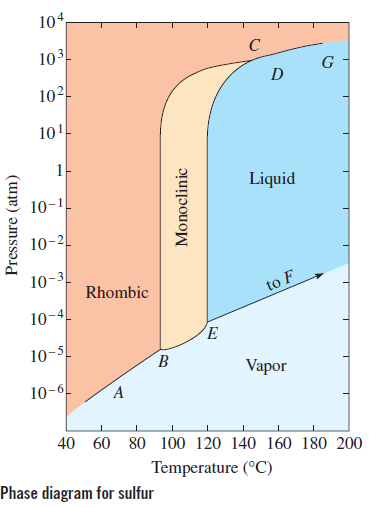
\includegraphics[scale=0.45]{sulfur_phase}

\begin{enumerate}[(a)]
\item Determine all triple points.
\item[]\tikz[baseline=1ex]\draw (0,0) rectangle (17cm,5ex);
\item Suppose a sulfur sample is at 1 atm and 140$^\circ$C. The sample is cooled to 80$^\circ$C at
constant pressure then subsequently, the pressure is decreased to 10$^{-3}$ atm at constant temperature.
What state of matter is sulfur?
\item[]\tikz[baseline=1ex]\draw (0,0) rectangle (17cm,5ex);
\end{enumerate}

\newpage

\noindent\textbf{Problem 2: Osmotic Pressure} Osmotic pressure is the minimum pressure
which needs to be applied to a solution to prevent the inward flow of its pure solvent
across a semipermeable membrane. (8 pts)

\begin{center}
  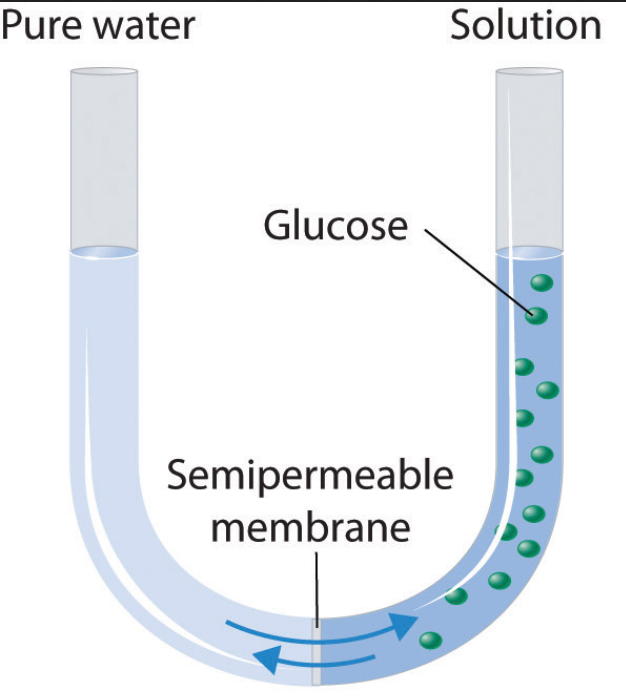
\includegraphics[scale=0.25]{osmotic_press}
\end{center}

\begin{enumerate}[(a)]
\item For the image above, there is pure water and glucose solutions separated by a
  semipermeable membrane. Describe what will happen to the water level of each solution
  once equilibrium is achieved.
\item[]\tikz[baseline=1ex]\draw (0,0) rectangle (17cm,30ex);
\item What is the osmotic pressure of a solution prepared by adding 10.35 g of
  sucrose (C$_{12}$H$_{22}$O$_{11}$) to water to make 175.0 mL of solution at 25.00$^\circ$C.
  \vspace{2in}
\item[]\tikz[baseline=1ex]\draw (0,0) rectangle (17cm,5ex);
\end{enumerate}

\newpage

\noindent\textbf{Problem 3: Heating Curve} Iodine (I$_2$) is a unique element in that the non-metallic
and dark-grey material is solid at room temperature. Suppose you have 115.0g of I$_2$ at room temperature
$25.0^\circ$C and heat the material to 175.5$^\circ$C. The melting and boiling points of I$_2$ are 114$^\circ$C
and 184$^\circ$C, respectively. Enthalpy of fusion and enthalpy of vaporization are 7.824 kJ/mol and
20.752 kJ/mol, respectively. Solid I$_2$ has specific heat of 0.427 J/(g $^\circ$C) and liquid I$_2$ has
specific heat of 2.150 J/(g $^\circ$C). (10 pts)

\begin{enumerate}[(a)]
\item Give a brief answer why I$_2$ is a solid at room temperature while Bromine (Br$_2$) is a gas.
\item[]\tikz[baseline=1ex]\draw (0,0) rectangle (17cm,10ex);
\item Draw a graph of the heating curve for I$_2$ described in the problem above. Label the y-axis as
  temperature ($^\circ$C) and the x-axis as heat added.
\item[]\tikz[baseline=1ex]\draw (0,0) rectangle (17cm,35ex);
\item Using the graph in (b), calculate the total heat in kJ required to heat 115.0g I$_2$ from 25.0$^\circ$C to
  175.5$^\circ$C.
  \vspace{3in}
\item[]\tikz[baseline=1ex]\draw (0,0) rectangle (17cm,5ex);
\end{enumerate}

\newpage

\noindent\textbf{Problem 4: Intermolecular Forces} For the following compounds:
H$_2$SO$_3$, C$_{10}$H$_{22}$ (decane), H$_2$O, NH$_3$, CH$_3$CF$_3$. Answer the
following questions. (10 pts)

\begin{enumerate}[(a)]
\item List out all types of intermolecular forces for the compounds listed above.
\item[]\tikz[baseline=1ex]\draw (0,0) rectangle (17cm,30ex);  
\item Rank from highest to lowest boiling point.
\item[]\tikz[baseline=1ex]\draw (0,0) rectangle (17cm,5ex);
\item Rank from highest to lowest vapor pressure.
\item[]\tikz[baseline=1ex]\draw (0,0) rectangle (17cm,5ex);
\item Rank from strongest to weakest intermolecular interactions.
\item[]\tikz[baseline=1ex]\draw (0,0) rectangle (17cm,5ex);
\item \textbf{Extra Credit (5 pts):} Dispersion is present in all materials. Provide both the
  textbook definition and Prof. Nguyen's landmark publication definition of dispersion.
  Include illustration if needed. No partical credit is given for this question.
\item[]\tikz[baseline=1ex]\draw (0,0) rectangle (17cm,50ex);
\end{enumerate}

\newpage

\noindent\textbf{Problem 5: Photoelectric Effect} When light shines on a metal, electrons can be ejected from
the surface of the metal in a phenomenon known as the photoelectric effect. You perform an experiment to
eject electrons from nickel (Ni) metal. It is known that a wavelength of 400 nm is the minimum energy to eject
an electron from Ni. (12 pts)
\\
\begin{enumerate}[(a)]
\item Determine the work function ($\Phi$), or the minimum energy in J to eject an electron, of the Ni metal.%
  \vspace{1.75in}
\item[]\tikz[baseline=1ex]\draw (0,0) rectangle (17cm,5ex);
\item How much energy in kJ is required to eject a mole of electrons from Ni metal? (Hint: One photon with
  enough energy ejects 1 electron.)
  \vspace{1.75in}
\item[]\tikz[baseline=1ex]\draw (0,0) rectangle (17cm,5ex);
\item What is the velocity of the electron if a photon with a frequency $1.5 \times 10^{15} \text{ Hz}$
  hits the surface of Ni metal and ejects an electron? The mass of an electron is $9.109 \times 10^{-31}$ kg.
  \vspace{1.75in}
\item[]\tikz[baseline=1ex]\draw (0,0) rectangle (17cm,5ex);
\end{enumerate}

\newpage

\noindent\textbf{Problem 6: Valence Bond Theory and Molecular Orbital Theory}
(10 pts)

\begin{enumerate}[(a)]
\item Draw the Lewis structure of \underline{P}O$_4^{3-}$. Indicate all resonance
  structures, resonance hybrid structure, structural geometry and electronic
  arrangement. For the underlined atom, indicate what hybridized orbital.
\item[]\tikz[baseline=1ex]\draw (0,0) rectangle (17cm,50ex);
\item Provide the definitions of valence bond theory and molecular orbital theory.
  What is the nuance difference between the two theories?
\item[]\tikz[baseline=1ex]\draw (0,0) rectangle (17cm,50ex);
\end{enumerate}

\newpage

\noindent\textbf{Problem 7: Limiting Reagent} Magnesium silicide (Mg$_2$Si) is a type of semiconductor.
However, it is highly reactive reactive with water (H$_2$O) according to the unbalanced chemical equation
(14 pts)
\begin{center}
  Mg$_2$Si(s) + H$_2$O(l) $\rightarrow$ Mg(OH)$_2$(aq) + SiH$_4$(g)
\end{center}

\begin{enumerate}[(a)]
\item Write the balanced chemical equation of the reaction above.
\item[]\tikz[baseline=1ex]\draw (0,0) rectangle (17cm,5ex);
\item Which reactant is the limiting if there are 50.0g H$_2$O(l) and 70.0g Mg$_2$Si(s)?
  \vspace{2in}
\item[]\tikz[baseline=1ex]\draw (0,0) rectangle (17cm,5ex);
\item How much Mg(OH)$_2$ in g is produced based on the amount of reactant in
  part (b)?
  \vspace{1.75in}
\item[]\tikz[baseline=1ex]\draw (0,0) rectangle (17cm,5ex);
\item What is the percent yield if a scientist collected 78.9g of Mg(OH)$_2$?
  \vspace{1.5in}
\item[]\tikz[baseline=1ex]\draw (0,0) rectangle (17cm,5ex);
\end{enumerate}

\newpage

\appendix

\section{Apppendix 2 - Formulas and Constants}

\begin{center}
  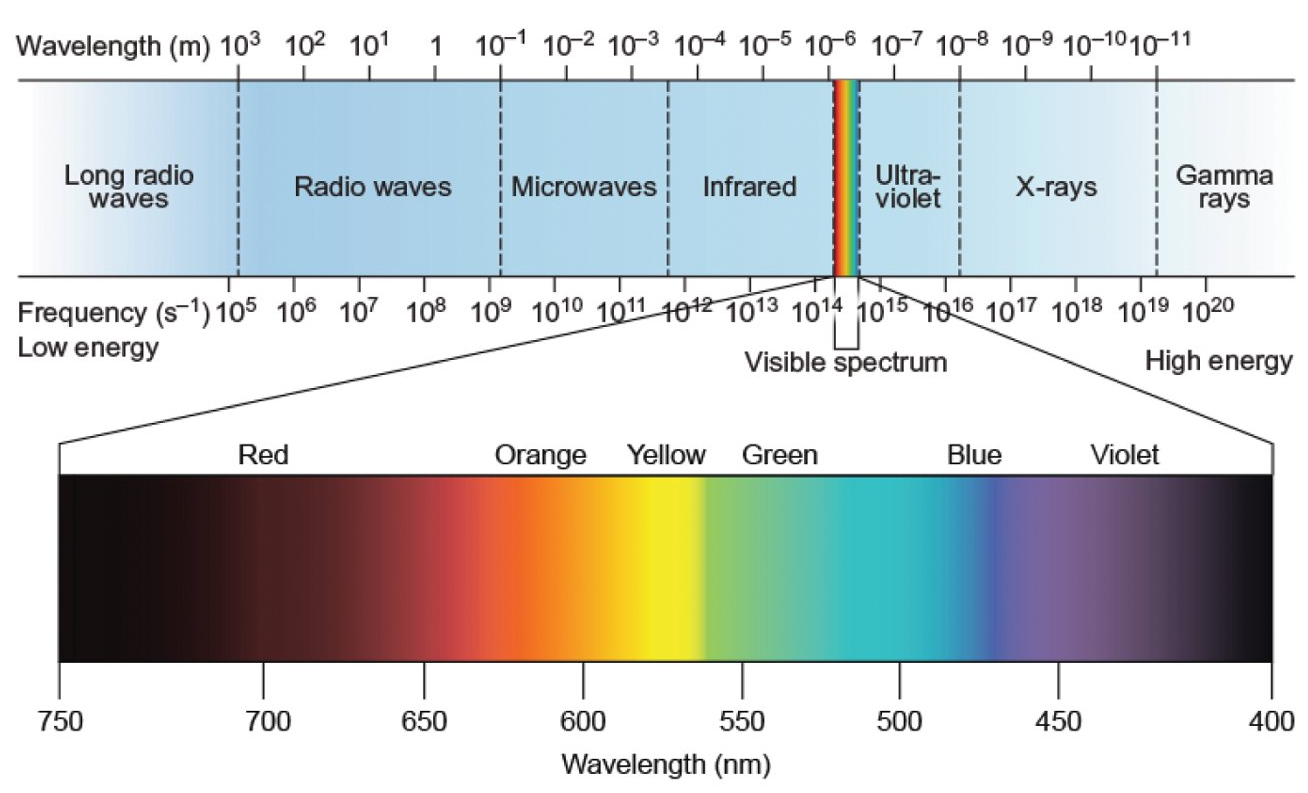
\includegraphics[scale=0.25]{electromag}
\end{center}

\begin{align*}
  c & = \lambda \nu \\
  E & = h\nu = \frac{hc}{\lambda} \\
  h & = 6.626 \times 10^{-34} \text{ J s} \\
  c & = 3.00 \times 10^{8} \text{ m/s} \\
  \text{KE} & = h\nu - \Phi \\
  \text{KE} & = \frac{1}{2} mv^2 \\
  m_\text{electron} & = 9.109 \times 10^{-31} \text{ kg} \\
  N_A & = 6.022 \times 10^{23} \text{particles/mol} \\
  q & = mc\Delta T \\
  q & = n\Delta H_\text{fus/vap} = m\Delta H_\text{fus/vap} \\
  \Pi & = iMRT \\
  R & = 8.3145 \text{J/(mol K)} = 0.08205 \text{L atm/(mol K)}
\end{align*}

\begin{center}
  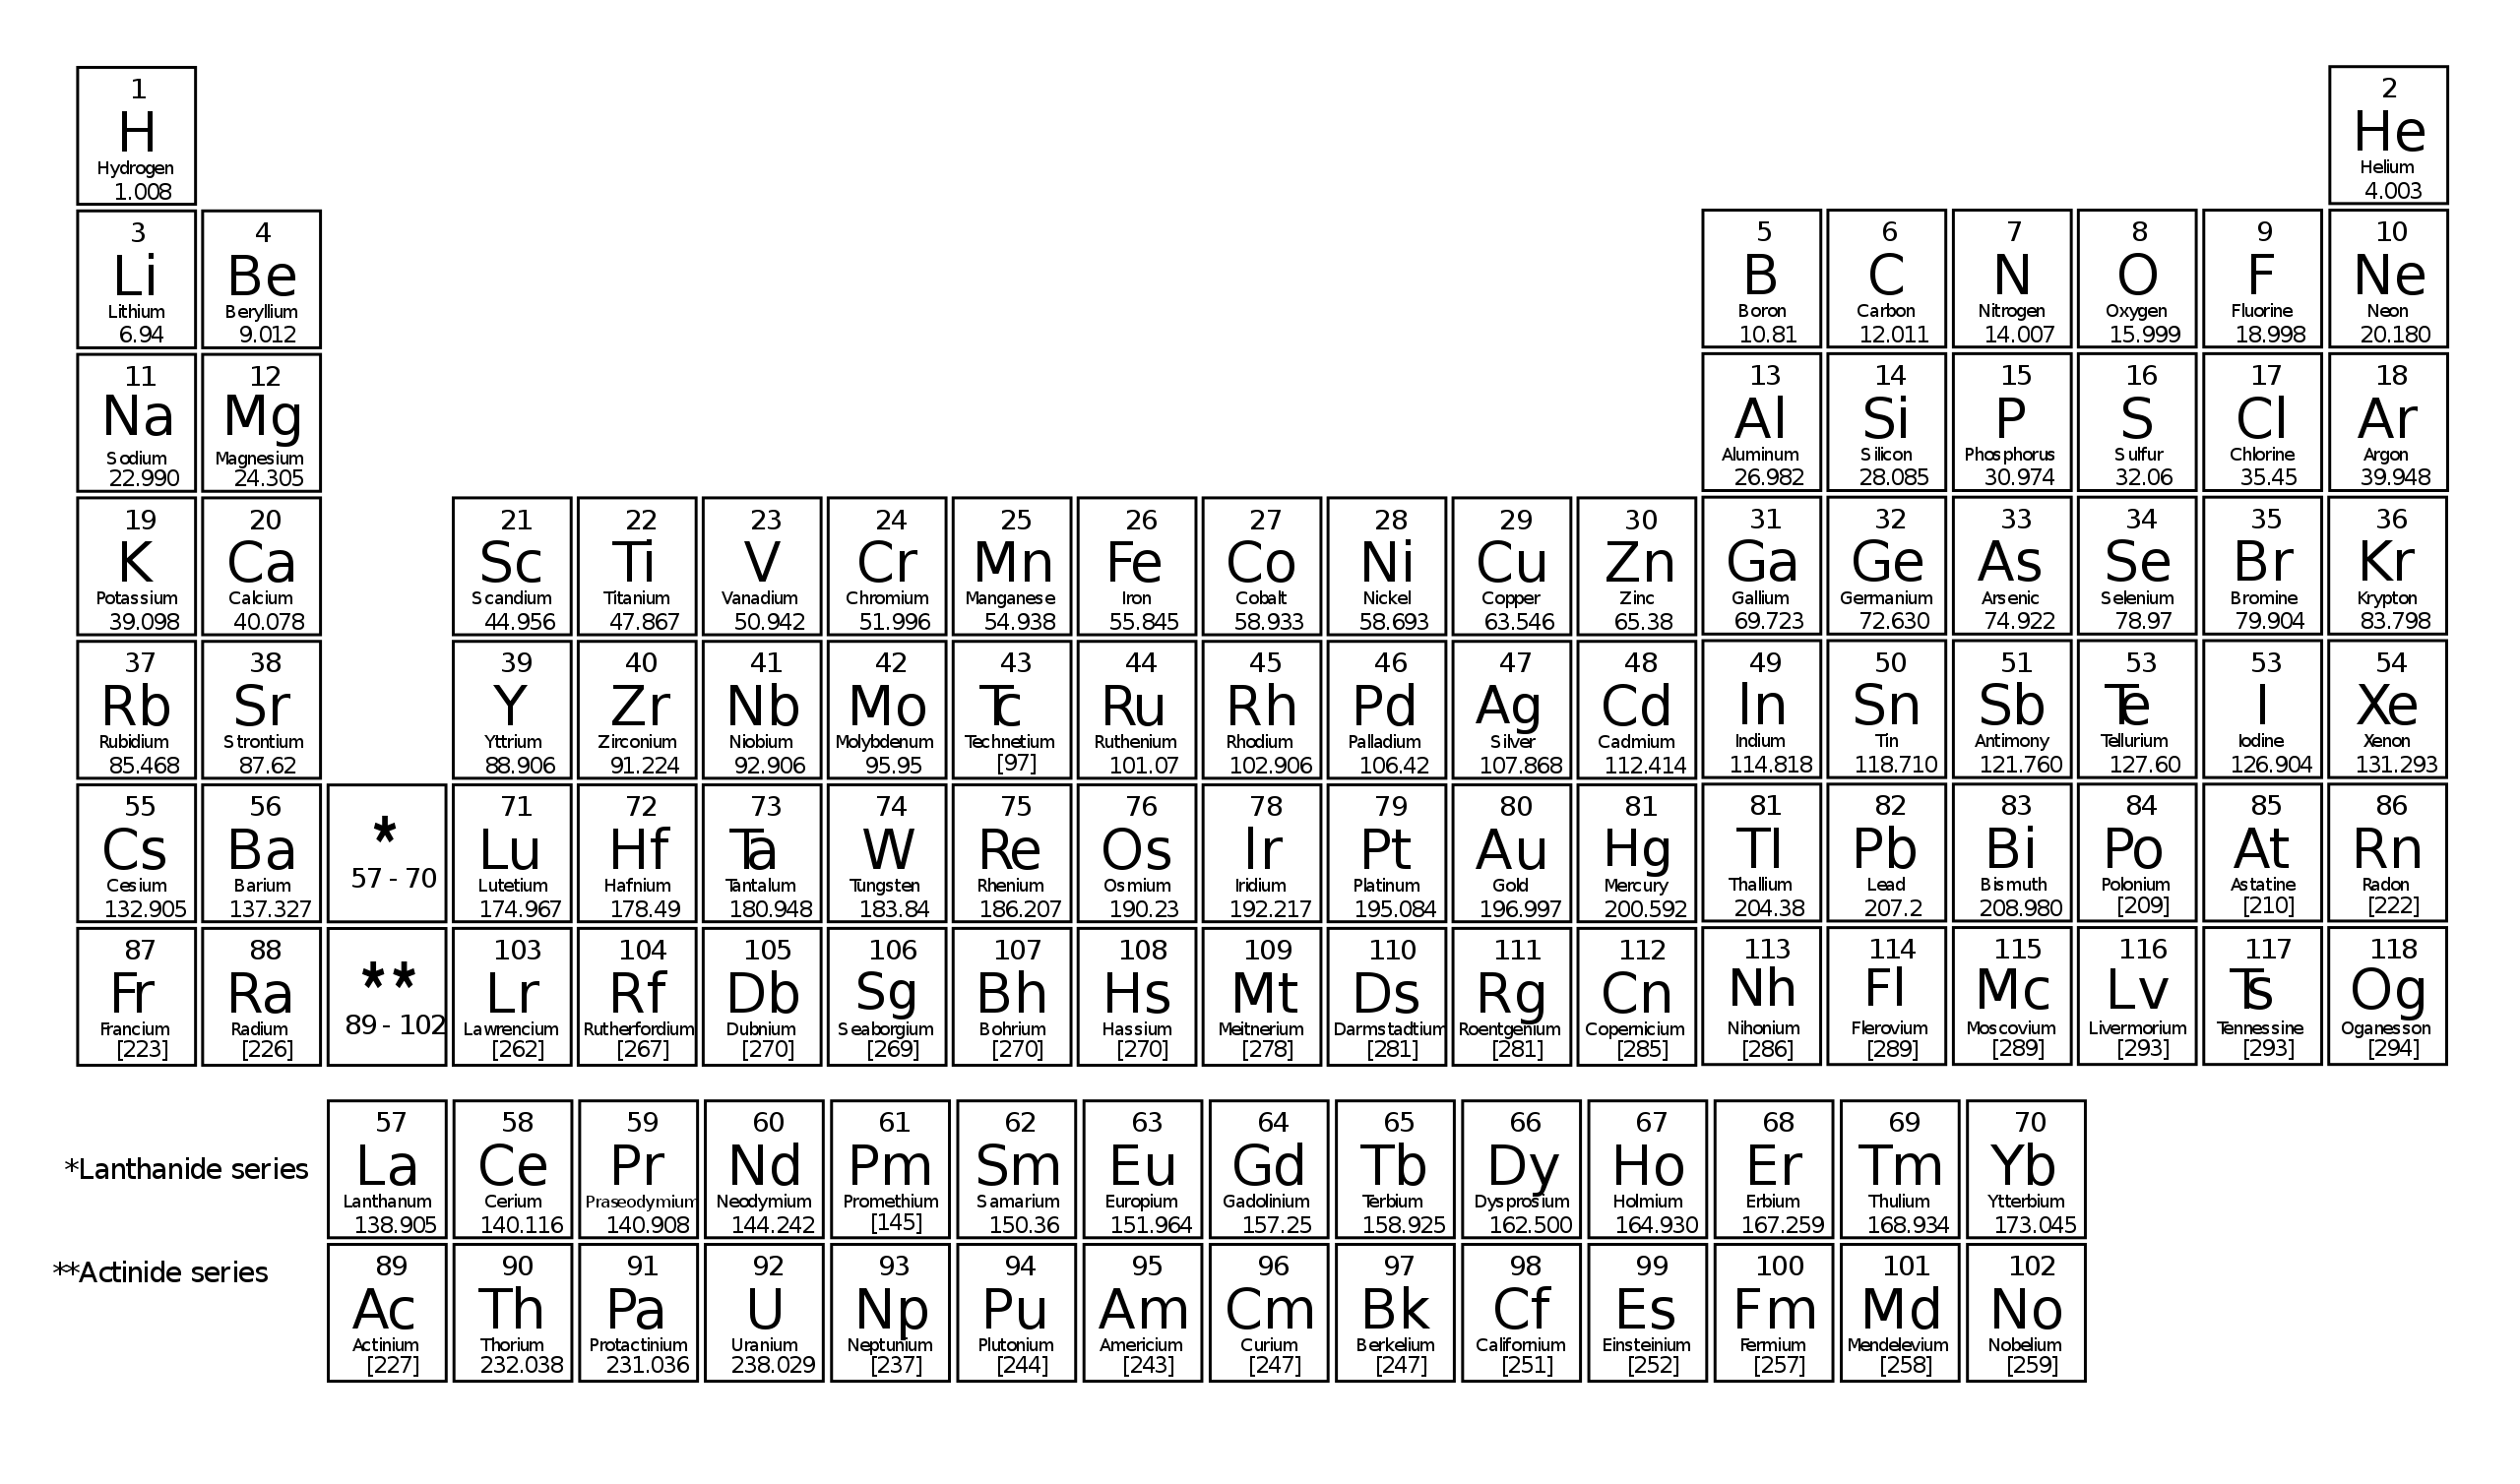
\includegraphics[scale=0.26,angle=90]{periodic_table}
\end{center}

\end{document}
